\documentclass[a4paper,12pt]{article} %размер бумаги устанавливаем А4, шрифт 12пунктов
\usepackage[utf8x]{inputenc}
\usepackage[english,russian]{babel}
\usepackage{cmap}
\usepackage{amssymb,amsfonts,amsmath,cite,enumerate,float,indentfirst} %пакеты расширений
\usepackage[pdftex]{graphicx} %вставка графики

\usepackage{color} %% это для отображения цвета в коде
\usepackage{listings} %% собственно, это и есть пакет listings
\definecolor{codegreen}{rgb}{0,0.6,0}
\definecolor{codegray}{rgb}{0.5,0.5,0.5}
\definecolor{codepurple}{rgb}{0.58,0,0.82}
\definecolor{backcolour}{rgb}{0.85,0.85,0.85}
 
\lstloadlanguages{C,make} 
\lstset{ %
extendedchars=\true,
inputencoding=utf8x,  
backgroundcolor=\color{white},   
commentstyle=\color{codegreen},
keywordstyle=\color{blue},
basicstyle=\fontsize{10}{12}\selectfont\ttfamily,
numberstyle=\tiny\color{codegray},
stringstyle=\color{codepurple},
breakatwhitespace=false,         
breaklines=true,                 
captionpos=t,                    
keepspaces=true,                 
numbers=left,                    
numbersep=5pt,                  
showspaces=false,                
showstringspaces=false,
showtabs=false,                  
tabsize=4,
frame=tb,
}

\newcommand{\myCodeInput}[3]{
{\bf #2}
\lstinputlisting[language=#1]{#3}
}


\graphicspath{ {images} }


\makeatletter
\renewcommand{\@biblabel}[1]{#1.} % Заменяем библиографию с квадратных скобок на точку:
\makeatother

\usepackage{geometry} % Меняем поля страницы
\geometry{left=2cm}% левое поле
\geometry{right=1.5cm}% правое поле
\geometry{top=1cm}% верхнее поле
\geometry{bottom=2cm}% нижнее поле

\renewcommand{\theenumi}{\arabic{enumi}}% Меняем везде перечисления на цифра.цифра
\renewcommand{\labelenumi}{\arabic{enumi}}% Меняем везде перечисления на цифра.цифра
\renewcommand{\theenumii}{.\arabic{enumii}}% Меняем везде перечисления на цифра.цифра
\renewcommand{\labelenumii}{\arabic{enumi}.\arabic{enumii}.}% Меняем везде перечисления на цифра.цифра
\renewcommand{\theenumiii}{.\arabic{enumiii}}% Меняем везде перечисления на цифра.цифра
\renewcommand{\labelenumiii}{\arabic{enumi}.\arabic{enumii}.\arabic{enumiii}.}% Меняем везде перечисления на цифра.цифра

\newcommand{\imgh}[3]{\begin{figure}[h]\center{\includegraphics[width=#1]{#2}}\caption{#3}\label{ris:#2}\end{figure}}

\begin{document}


\begin{titlepage}
\newpage

\begin{center}
Министерство науки и высшего образования Российской Федерации \\
Новосибирский государственный технический университет
\end{center}

\vspace{8em}

\begin{center}
\Large Управление ресурсами в вычислительных системах \\ 
\end{center}

\vspace{2em}

\begin{center}
\textsc{\textbf{Лабораторная работа №3}}
\end{center}

\vspace{6em}



\newbox{\lbox}
\savebox{\lbox}{\hbox{Пупкин Иван Иванович}}
\newlength{\maxl}
\setlength{\maxl}{\wd\lbox}
\hfill\parbox{11cm}{
\hspace*{5cm}\hspace*{-5cm}Группа:\hfill\hbox to\maxl{ПМ-13}\\
\hspace*{5cm}\hspace*{-5cm}Студенты:\hfill\hbox to\maxl{Исакин Д.А.\hfill}\\
\hspace*{5cm}\hspace*{-5cm}\hfill\hbox to\maxl{Вострецова Е.В.\hfill}\\
\hspace*{5cm}\hspace*{-5cm}Преподаватели:\hfill\hbox to\maxl{Стасышин В.М.\hfill}\\
\hspace*{5cm}\hspace*{-5cm}\hfill\hbox to\maxl{Сивак М.А.\hfill}\\
}


\vspace{\fill}

\begin{center}
Новосибирск \\2024
\end{center}

\end{titlepage}



\newpage
\begin{Large}
\textbf{1. Условие (Вариант №1)}\\
\end{Large}
	Исходный процесс создает два программных канала К1 и К2 и порождает
новый процесс Р1, а тот, в свою очередь, еще один процесс Р2, каждый из которых
готовит данные для обработки их основным процессом. Подготавливаемые данные
процесс Р1 помещает в канал К1, а процесс Р2 в канал К2, откуда они процессом Р1
копируются в канал К1 и дополняются новой порцией данных. Схема
взаимодействия процессов, порядок передачи данных в канал и структура
подготавливаемых данных показаны ниже:\\
\begin{center}
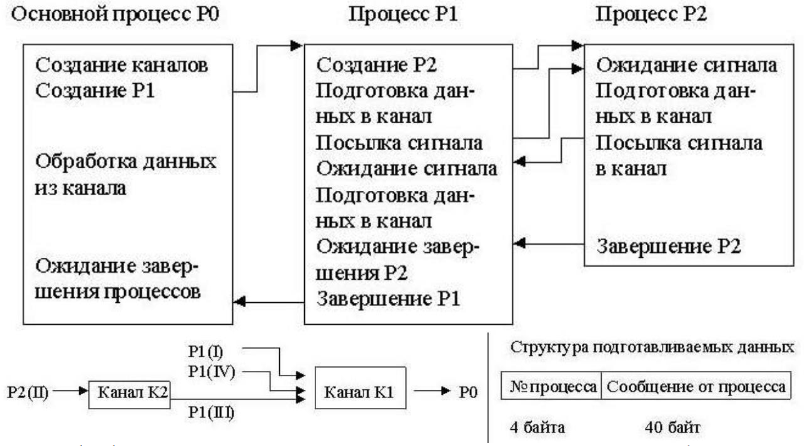
\includegraphics[width=1.0\linewidth]{cond.png}
\end{center}
	Обработка данных основным процессом заключается в чтении информации из
программного канала К1 и печати её. Кроме того, посредством выдачи сообщений
необходимо информировать обо всех этапах работы программы (создание процесса,
завершение посылки данных в канал и т.д.).

\newpage
\begin{Large}
\textbf{2.Анализ задачи}\\
\end{Large}

Создаём каналы K1 и K2 и порождаем процесс P1 и в процессе P1 пораждаем дочерний процесс P2\\
Для процессов\\
\textbf{P0:}
\begin{enumerate}
	\item Читаем данные из канала и выводим их на экран. Чтение производим по сигналу от 			дочернео процесса о том, что данные готовы
	\item Ожидаем завершение процесса P1
\end{enumerate}
\textbf{P1:}
\begin{enumerate}
	\item Создаем процесс Р2
	\item Готовим данные от Р1 и отправляем их в К1. После посылаем сигнал Р0
	\item Ждем от Р2 сигнала готовности
	\item Читаем данные из К2 и пишем их в К1. Посылаеп сигнал Р0
	\item Модификация данных. Пишем в К1. Посылаем Р0 сигнал готовности. После сигнал завершения
\end{enumerate}
\textbf{P2:}
\begin{enumerate}
	\item Готовим данные
	\item Пишем в К2
\end{enumerate}
\newpage

\begin{Large}
\textbf{3.Используемые програмные средства.}\\
\end{Large}

\begin{lstlisting}[language=C]
int fork(); - порождение процесса-потомка
int pipe(int[2]); - порождение канала
int fclose(const char*file); - закрытие файла или канала
int kill(pid_t pid, int sygnal); - передача сигнала
int read(int fd, char *data, int dataSize); - чтение из канала файла
int waitpid(pid_t pid,int *status, NULL); - ожидание завершения процесса-потомка
int getpid(); - определение pid текущего процесса
int getppid(); - определение процесса родителя 
int sleep(int seconds); - остановка процесса на n секунд
\end{lstlisting}

\begin{Large}
\textbf{4. Спецификация}\\
\end{Large}
\begin{itemize}
\item Программа находится в папке ~/lab3
\item Чтобы собрать программу нужно ввести make
\item Чтобы запустить программу, нужно использовать команду “./lab3”
\item В результате работы программы, будет показаны сообщения о действиях процессов P0, P1 и P2 такие как создание / завершение процессов, чтение файла процессом P0. Завершение процессов потомков.  
\end{itemize}

\begin{Large}
\textbf{5. Результат работы программы}\\
\end{Large}

\begin{lstlisting}
P0: Try to create K1
P0: K1 create success
P0: Try to create K2
P0: K2 create success

P0: Try to create P1
P1: P1 create sucess. pid(P1) = 0
P1: Try to create P2
P1(1): Data wreaten and send to K1
P0: pid = 148244, data = Data: P1
P2: P2 create sucess. pid(P2) = 0
P2(2): Data writen and sended to K2
P1: Process P2 was end correct
P1(3): Data from P2 got and written to K1 and sended
P1(4): Data P1 modifie and send to K1
P0: break;
P0: Process P1 was end correct
\end{lstlisting}

\newpage

\begin{Large}
\textbf{6. Исходный код}
\end{Large}

\myCodeInput{c}{main.c}{main.c}
\myCodeInput{make}{makefile}{makefile}
\end{document}

